\begin{figure}[H]
\centering
\includegraphics[page=6,width=0.47\textwidth]{\FCNCFigures/tthML/showFake/faketau/postfit/NOMINAL/reg1l1tau1b2j_ss_vetobtagwp70_highmet/BDTG_test.pdf}
\includegraphics[page=6,width=0.47\textwidth]{\FCNCFigures/tthML/showFake/faketau/postfit/NOMINAL/reg1l1tau1b2j_ss_vetobtagwp70_highmet/dphitauetmiss.pdf}
\\
\includegraphics[page=6,width=0.47\textwidth]{\FCNCFigures/tthML/showFake/faketau/postfit/NOMINAL/reg1l1tau1b2j_ss_vetobtagwp70_highmet/drlb.pdf}
\includegraphics[page=6,width=0.47\textwidth]{\FCNCFigures/tthML/showFake/faketau/postfit/NOMINAL/reg1l1tau1b2j_ss_vetobtagwp70_highmet/drltau.pdf}
\\
\includegraphics[page=6,width=0.47\textwidth]{\FCNCFigures/tthML/showFake/faketau/postfit/NOMINAL/reg1l1tau1b2j_ss_vetobtagwp70_highmet/drtaub.pdf}
\includegraphics[page=6,width=0.47\textwidth]{\FCNCFigures/tthML/showFake/faketau/postfit/NOMINAL/reg1l1tau1b2j_ss_vetobtagwp70_highmet/drtaujmin.pdf}
\\
\caption{$l\thad$ 2j信号区中各变量的分布图,图中信号为tuH耦合。}
\label{fig:var_reg1l1tau1b2j_ss_vetobtagwp70_highmet_1}
\end{figure}
\begin{figure}[H]
\centering
\includegraphics[page=6,width=0.47\textwidth]{\FCNCFigures/tthML/showFake/faketau/postfit/NOMINAL/reg1l1tau1b2j_ss_vetobtagwp70_highmet/drtautau.pdf}
\includegraphics[page=6,width=0.47\textwidth]{\FCNCFigures/tthML/showFake/faketau/postfit/NOMINAL/reg1l1tau1b2j_ss_vetobtagwp70_highmet/etamax.pdf}
\\
\includegraphics[page=6,width=0.47\textwidth]{\FCNCFigures/tthML/showFake/faketau/postfit/NOMINAL/reg1l1tau1b2j_ss_vetobtagwp70_highmet/etmiss.pdf}
\includegraphics[page=6,width=0.47\textwidth]{\FCNCFigures/tthML/showFake/faketau/postfit/NOMINAL/reg1l1tau1b2j_ss_vetobtagwp70_highmet/lep_pt_0.pdf}
\\
\includegraphics[page=6,width=0.47\textwidth]{\FCNCFigures/tthML/showFake/faketau/postfit/NOMINAL/reg1l1tau1b2j_ss_vetobtagwp70_highmet/met_sigma.pdf}
\includegraphics[page=6,width=0.47\textwidth]{\FCNCFigures/tthML/showFake/faketau/postfit/NOMINAL/reg1l1tau1b2j_ss_vetobtagwp70_highmet/mjjmin.pdf}
\\
\caption{$l\thad$ 2j信号区中各变量的分布图,图中信号为tuH耦合。}
\label{fig:var_reg1l1tau1b2j_ss_vetobtagwp70_highmet_2}
\end{figure}
\begin{figure}[H]
\centering
\includegraphics[page=6,width=0.47\textwidth]{\FCNCFigures/tthML/showFake/faketau/postfit/NOMINAL/reg1l1tau1b2j_ss_vetobtagwp70_highmet/mtaujmin.pdf}
\includegraphics[page=6,width=0.47\textwidth]{\FCNCFigures/tthML/showFake/faketau/postfit/NOMINAL/reg1l1tau1b2j_ss_vetobtagwp70_highmet/phicent.pdf}
\\
\includegraphics[page=6,width=0.47\textwidth]{\FCNCFigures/tthML/showFake/faketau/postfit/NOMINAL/reg1l1tau1b2j_ss_vetobtagwp70_highmet/t1mass.pdf}
\includegraphics[page=6,width=0.47\textwidth]{\FCNCFigures/tthML/showFake/faketau/postfit/NOMINAL/reg1l1tau1b2j_ss_vetobtagwp70_highmet/tau_pt_0.pdf}
\\
\includegraphics[page=6,width=0.47\textwidth]{\FCNCFigures/tthML/showFake/faketau/postfit/NOMINAL/reg1l1tau1b2j_ss_vetobtagwp70_highmet/tautaumass.pdf}
\includegraphics[page=6,width=0.47\textwidth]{\FCNCFigures/tthML/showFake/faketau/postfit/NOMINAL/reg1l1tau1b2j_ss_vetobtagwp70_highmet/tautauvispt.pdf}
\\
\caption{$l\thad$ 2j信号区中各变量的分布图,图中信号为tuH耦合。}
\label{fig:var_reg1l1tau1b2j_ss_vetobtagwp70_highmet_3}
\end{figure}
\begin{figure}[H]
\centering
\includegraphics[page=6,width=0.47\textwidth]{\FCNCFigures/tthML/showFake/faketau/postfit/NOMINAL/reg1l1tau1b2j_ss_vetobtagwp70_highmet/ttvismass.pdf}
\includegraphics[page=6,width=0.47\textwidth]{\FCNCFigures/tthML/showFake/faketau/postfit/NOMINAL/reg1l1tau1b2j_ss_vetobtagwp70_highmet/wmass.pdf}
\\
\includegraphics[page=6,width=0.47\textwidth]{\FCNCFigures/tthML/showFake/faketau/postfit/NOMINAL/reg1l1tau1b2j_ss_vetobtagwp70_highmet/x1fit.pdf}
\includegraphics[page=6,width=0.47\textwidth]{\FCNCFigures/tthML/showFake/faketau/postfit/NOMINAL/reg1l1tau1b2j_ss_vetobtagwp70_highmet/x2fit.pdf}
\\
\caption{$l\thad$ 2j信号区中各变量的分布图,图中信号为tuH耦合。}
\label{fig:var_reg1l1tau1b2j_ss_vetobtagwp70_highmet}
\end{figure}
